\chapter{Introduction}
Transcriptome is the total set of transcripts, or mRNA and other non-coding RNAs
within the cell. Unlike the genome, which acts as a template for different life
forms, transcriptome can vary according to the context, i.e. specific tissues or
external stimuli. In addition, the dynamics of gene expression roughly coincides 
with that of the cellular phenotype, which makes the study of transcriptome 
especially promising. In this chapter, we summarize the current knowledge about
the cellular response to stimulus, highlight the need to approach the problem
by in a theoretical way, and provide both the dynamic and network representation
of the gene regulatory networks.

\section{Cellular signal processing}
Cells are the building blocks of all living organisms except viruses. As an 
independent functional unit, individual cells sense the environmental cues 
(such as cytokine or growth factor stimulation, extracellular matrix interactions, DNA damage, or osmotic stress) by the membrane receptors. The latter
then activate a cascade of protein reaction and modification in the cytoplasm,
which leads to the gene regulation in the nucleus being triggered by 
DNA-binding proteins, i.e. transcription factors. Post-transcriptional
regulations again forms feedback loops at various levels, which act upon the
upstream signaling proteins (\ref{fig:signal_flow}).

\begin{figure}[!ht]
\begin{center}
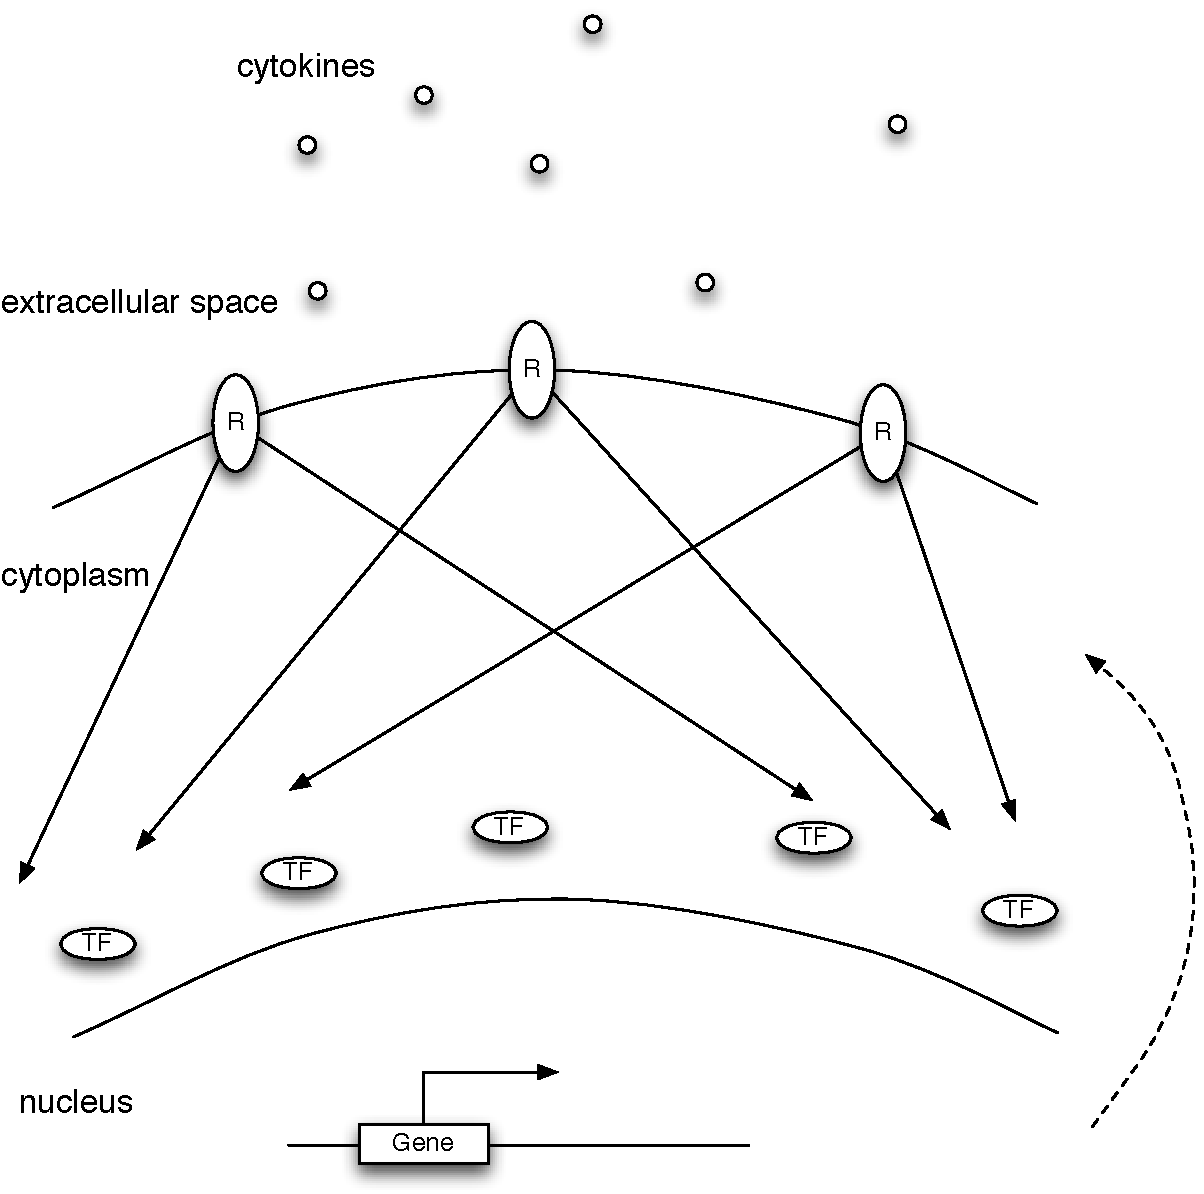
\includegraphics[width=\textwidth]{signal_flow.pdf}
\end{center}
\caption[Signal flow]{{\bf Schematic view of signal flow from membrane 
receptors to transcription factors in the cell.}
}
\label{fig:signal_flow}
\end{figure}

The last decades have witnessed the transition from a classical view of 
simple linear signaling pathways
to the idea of an intertwingled signaling network coordinating multiple 
pathways~\citep{Kholodenko2012}. Techniques as yeast two hybrid system 
and mass spectrometry based
proteomics have greatly enhanced the ability to map the components of such 
signal transduction networks. Despite the inherent large number of false
positive hits from such high-throughput studies, efforts have been devoted
to collect different sources of protein-protein interaction 
(PPI) data, such as BioGRID%
~\citep{Stark2006} and STRING~\citep{Szklarczyk2011}. Recently, the HIPPIE
database~\citep{Schaefer2012} was proposed to integrate multiple experimental PPI
data sources and assign a score to each interaction. This
score measures the number of publications reporting a certain
interaction, the quality of the experimental technique used
to detect this interaction, and how conserved this particular
interaction is across species. Such efforts have greatly 
contributed to the current knowledge of protein interactions
and therefore the backbone of the signal propagation network.

By further investigating the time-resolved phosphorylation
events, one gets additional information about some general
and context-specific mechanisms of signal flow.
For instance, in a phospho-proteomic study of 
HeLa cells stimulated with epidermal growth factor (EGF)~%
\citep{Olsen2006},
it was found that the majority of proteins contain multiple 
phosphorylation sites showing different kinetics, which 
suggests that they serve as platforms for integrating 
signals. As another example, a phospho-proteomic analysis
of human embryonic stem cell differentiation in response
to different stimuli~\citep{Ribbolt2011} reveals interesting
dynamic phosphorylation of DNA methyltransferases, which
regulate several pluripotency marker genes and thereby 
providing a link between the differential signal and the
downstream transcriptional machinery.

\section{Predictive analysis and systems biology}

\section{Dynamical system}

\section{Network}
